\documentclass[10pt, reqno]{amsart}
\usepackage{macros}
\AtBeginEnvironment{quote}{\singlespace\vspace{-\topsep}\small}
\AtEndEnvironment{quote}{\vspace{-\topsep}\endsinglespace}
\raggedbottom

\title{What Works the Best for Boston: Boston Mechanism, Deferred Acceptance, and More}
\author{Ryan Liu and Lotus Xia}
\date{\today}


\begin{document}
\maketitle

% \section{Notes}
% assignment policy: \url{https://www.bostonpublicschools.org/cms/lib/MA01906464/Centricity/Domain/187/DiscoverBPS%2021%20English.pdf}

% Students can select all Boston high schools. 33 high schools, 17 open enrollment HS. In simulation, use 27 high school. School preference is based on priority scores of each student: 1. sibling priority (attribute 2 points), and 2. east Boston/ Non-est Boston priority (attribute 1 point). The schools use a random tie breaker for students with the same priority score. 


% One school choice strategy is to find a school you like that is undersubscribed and put it as a top choice, OR, find a school that you like that is popular and put it as a first choice and find a school that is less popular for a “safe” second choice. (Pathak and Sonmez 2008)


\section{Introduction}

School choice problems have attracted significant attention in theoretical, experimental, and empirical literature \citep{chen2013boston,abdulkadirouglu2003school,kapor2020heterogeneous}. It is nearly a consensus in theoretical market design literature that mechanisms that incentivize truthful reporting of preference orders are preferable \citep{azevedo2019strategy}. Among them, Deferred Acceptance (DA for simplicity) is strongly advocated for its strategyproofness and stability \citep{pathak2008leveling}. Despite its popularity among theoretical literature, DA is far from the go-to option in real life. As of 2018, Boston is the only city in the U.S. that employs the canonical version of DA; New York City and Chicago adopt variations of DA that are not fully strategyproof. On the contrary, the Boston Mechanism (Boston for simplicity), one the most manipulable and unstable mechanisms, is more widely adopted by many major cities and regions in the U.S., including Denver, Minneapolis, Tampa-St. Petersburg Metropolitan Area, and Miami-Dade \citep{agarwal2018demand}. 

This poses some importance questions both theoretically and empirically: what are the costs and benefits of DA and Boston? What mechanism is the most desirable by public school systems? A seminal paper by \cite{pathak2008leveling} points out that the Boston Mechanism puts students from different socioeconomic classes on an uneven playing field: families that strategize effectively gain an advantage at the expense of families that do strategize and submit their true preferences. This put students from different socioeconomic background on an uneven playing field, since underprivileged students may lack the time and resource to study the optimal strategies in the Boston Mechanism. On the other hand, \cite{agarwal2018demand} provide a different perspective on the same topic. They estimating the underlying distribution of student preference from school admission data and point out that the Boston Mechanism is preferred by the average student to the Deferred Acceptance mechanism in equilibrium. 

\TODO{maybe add a bit more about why we care about this topic?} 

In this paper, we give a simple and preliminary cost and benefit analysis about DA and Boston using a simulation based on Boston public high school admission systems. Our goals are two-folds.
First, we compare DA and Boston along three dimensions: 1) fairness, 2) welfare, 3) stability, and hope to provide a more holistic view of the cost and benefit analysis. Second, we explore the Chinese Parallel Mechanism, which stands in between Boston and DA from a theoretical perspective, along the same three dimensions. 

\section{Mechanism Under Consideration}

\subsection{Deferred Acceptance and the Boston Mechanism}

We have studied DA and Boston extensively in lecture, problem sets, and embedded EthiCS seminar, so we refrain from restating the detailed steps in these two mechanisms in the interest of space. We highlight some theoretical results that are particularly relevant for our analyses below. 

First, the student-proposing DA is student-optimal among all stable matchings. Second, the Boston Mechanism results in the Pareto-optimal assignment among all matchings. Third, there is theoretical evidence that student-optimal stable mechanism outcomes may produce large welfare losses \cite{kesten2010school}.

\subsection{The Chinese Parallel Mechanism}
The comparison and contrast between DA and Boston naturally bring us to a third potential mechanism, the Chinese Parallel Mechanism, which is a essentially combination of the Boston Mechanism and Deferred acceptance. 

Chinese Parallel is a popular centralized mechanism used in Chinese college admission process---employed by 22 out of 34 provincial administrative regions as of 2012. For instance, Shanghai switched from the sequential mechanism (which is similar to the Boston Mechanism) to Chinese Parallel in 2008 and received positive feedback---there is 40.6\% decrease in the number of students who refused to go to the universities they were matched with.

The mechanism is as follows.

\begin{enumerate}
  \item Round 1: Each student lists her $e$ favorite schools. Each school lists it preference ordering for all student. We run Deferred Acceptance based on the incomplete preference orders from students and the complete preference orders from school. If a student is rejected by all of the $e$ schools, she remains unassigned in this round, and does not make any application until the next round. The resulting matches from Deferred Acceptance are final, and are not subject to change any more in future rounds. The capacity of each school is reduced by the number of students it gets this round. 

  \item Round $k$: Each unassigned student lists her $ke+1$-th through $(k+1)e$-th favorite schools. We again run Deferred Acceptance based on this set of incomplete student preference orders, the set of complete school preference orders, and the updated school capacity. Students rejected by all of her $ke + e$ through $(k+1)e$ choices remain unassigned in this round and cannot make any applications until the next round. All resulting matches at the end of this round are finalized. 

  \item The algorithm terminates when all students have been assigned to a school.
\end{enumerate}
The schools each student applies to in each round are referred to as ``parallel schools.'' 

We note that the Chinese Parallel Mechanism is identical to Deferred Acceptance when $e = \infty$ and is identical to the Boston Mechanism when $e = 1$. Later on, we use Chinese Parallel Mechanism to refer to mechanisms where $e \not=1$ and $e\not = \infty.$

In our simulation, we run 3 rounds of Chinese Parallel. In round 1, students apply to their 3 favorite schools; in round 2, students apply to their 4-6 choices; finally, in round 3, students apply to the rest of her schools. 

Theoretically, DA is more stable than Chinese Parallel, which is more stable than the Boston Mechanism, whereas the Boston Mechanism is more efficient than the Chinese Parallel, which is more efficient than DA. It follows quite intuitively that, while the Boston Mechanism maximizes the number of students receiving their first choices, the Chinese Parallel maximizes the number of students receiving their first $e$ choices 
\citep{chen2013boston}. Finally, Chinese Parallel elicits more truth-telling from, and therefore less manipulable by, students than the Boston Mechanism.

\section{Simulation}
We set up the simulation to closely follow the institutional setting in the Boston school choice system. To reduce the simulation difficulty, we focus on high school admissions. Boston's assignment of high schools is city-wide, in the sense that all students, regardless of school district, are eligible to all high schools in Boston.

There are a total of 33 high schools in Boston, 17 of which are open for general enrollment (``open enrollment schools''). The remaining 16 schools requires additional application requirements or special admission. We take the institutional details of these 17 open enrollment schools for our simulation. The number of students in our simulation equals 1880, which is the estimated capacity of 9th grade in these 17 school. As a comparison, there are approximately 4000 rising 9th graders in Boston Public high school system.\footnote{Boston Public School at a Glance, 2019-2020, \url{https://www.bostonpublicschools.org/cms/lib/MA01906464/Centricity/Domain/187/BPS\%20at\%20a\%20Glance\%202019-20\_FINAL.pdf}} In each simulation iteration, we randomly draw 20\% of the students to be sophisticated, and the rest are sincere. Sophisticated students strategize and may choose to misreport their true preference in Boston and Chinese Parallel. They report true preference in DA in our simulation since it is a dominant strategy to do so. We later change the percentage of sophisticated students to 80\% to study the effect on matching results.

\subsection{School Preference}
Schools rank students based on their ``priority'' scores. We focus on two types of priorities that affect admission into 9th grade, namely sibling priority and geographic priority. First and foremost, student $i$ has a higher priority at school $j$ if said students has a sibling currently enrolled in school $j$. This policy is to keep families together in the same school if that is what parents prefer. Second, given Boston's unique geography, students who live in East Boston are given priority to schools in East Boston, and students who live outside of East Boston are given priority to schools outside of East Boston. Only one school among the 17 open enrollment schools are located in East Boston area. Schools has a lexicographic preference of sibling priority to geographic priority. 

We attempt to simulate the school preference in the following steps:
\begin{enumerate}
  \item For each student, randomly draw whether she has a proper-age-sibling with probability 0.3. Randomly assign the sibling to enroll in one of the 17 schools with equal probability. 
  \item For each student, randomly draw whether she lives in East Boston with probability 0.1.\footnote{The East Boston area is approximately $1/10$ of the total area of Boston on the map.}
  \item For each pair of student $i$ and school $j$, compute the priority score as $2\times \text{sibling priority} + \text{geography priority}$. 
  \item Generate the cardinal utility of school $j$ for getting student $i$ as the priority score plus a random noise drawn from $U[0,1]$. Note that the random noise never puts students in a different priority bucket. 
  \item The preference order of each school is then computed based on the cardinal utility. 
\end{enumerate}

\subsection{Student Preference}
Schools rank students based on their education quality. On the official guide to Boston Public School choice, each high school is given a ``SQF Tier'' as a measure of the overall quality of the school. The official guide suggests that families should use the SQF score to better inform themselves and make customized school choice. The SQF score is from 1 to 4, with 1 being the most favorable rating. 

Based on the SQF score, we generate student preference in the following steps:
\begin{enumerate}
  \item Each school is assigned a quality score equal to $10 - \text{its SQF score}$, so that higher number is better. 
  \item For each pair of student $i$ and school $j$, compute the cardinal utility of student $i$ for getting into school $j$ as the quality score plus a random noise drawn from $N(0,1)$. 
  \item The preference order of each student is then computed based on the cardinal utility. 
\end{enumerate}

\subsection{Misreport}

Sophisticated students may choose to misreport in Boston and Chinese Parallel. 

In fact, West Zone Parents Group (WZPG), a well-informed group that regularly meet prior to admission time to discuss Boston school choice recommends two types of strategies to its members \citep{pathak2008leveling}:
\begin{quote}
One school choice strategy is to find a school you like that is undersubscribed and put it as a top choice, OR, find a school that you like that is popular and put it as a first choice and find a school that is less popular for a “safe” second choice.    
\end{quote}

We closely follow these suggestions and simulated two types of misreports under the Boston Mechanism. 
\begin{enumerate}
  \item Student $i$ looks at her top 3 choices and checks which school is ``safe.'' She reports her favorite safe school as her top choice, followed by all the other schools in her true preference order. If none of the top 3 choices are safe, then she report all preferences truthfully. 
  \item Student $i$ truthfully reports her first choice. She then looks at her second through fifth choices, and reports her favorite safe school among them as second choice. She then truthfully reports the rest of her preference. Again, if none of the 4 schools are safe, then she reports all preferences truthfully. 
\end{enumerate}

In both cases, a school $j$ is \textit{safe} for student $i$ if, under truthful reporting by everyone, $i$ is reasonably confident to get accepted by school $j$ as long as student $i$ lists school $j$ as first choice in the Boston Mechanism. In our simulation, we compute \textit{number of competitors} as the number of students who like school $j$ the most under true preference and are preferred by school $j$ to student $i$. We generate a \textit{perceived number of competitors} as the number of competitors plus a random noise drawn from $N(0,5)$. If the perceived number of competitors is smaller than the capacity of school $j$, then $j$ is considered safe for $i$. 

Under Chinese Parallel, all sophisticated students adopt the following misreport. 
\begin{enumerate}
	\item Students $i$ truthfully reports her first and second choice, but report a safe school as her third choice. Where ``safe'' is as defined above. To do this, she looks at her third through fifth choice on her true preference list, and report her favorite safe school among them as the third choice. She then truthfully reports the rest of her preference. Again, if none of the 3 schools are safe, then she reports all preferences truthfully. 
\end{enumerate}

This misreport is inspired by an equilibrium analysis by \citep{chen2013boston}. The intuition is simple. In Chinese Parallel, the first $e$ choices are crucial, just as the first choice is crucial in Boston. Students have incentives to guarantee a seat at an unpopular, but somewhat desirable school, by ranking it among the first set of parallel schools. This strategy leaves students with some chances to obtain a more preferred school, while prevent them from ending up in an undesirable school.\footnote{We searched in Baidu, the largest search engine in China, for college admission strategies under Chinese Parallel, but found no substantive suggestions on ways to misreport preferences and game the system. This is quite surprising. It is possible that these strategies are considered secretive and are only shared among a group of elite high schools.} 

We make two notes about these three misreports. 
First, it seems unrealistic for sophisticated students to have complete knowledge over 1) who list school $j$ as first choice and 2) who are preferred by school $j$, though families may have some estimates of the popularity of each school as well as the relative priority of themselves among all applicants.We attempt to simulate the inaccurate estimates by the perceived number of competitors. 
Second, the strategies does not take into account equilibrium effect. For instance, student $i$ may theoretically end up rejected by school $j$ even if $j$ is safe for $i$, since other students may misreport their top choice and make school $j$ more popular. In fact, many existing papers on school choice study the Bayes-Nash equilibrium property of different mechanisms. However, we believe that it is unlikely that families in real life have a good understanding of the Nash Equilibrium of a game involving thousands of students and tens of school. A naive strategy that only looks one step ahead may be more realistic in this setting. 

In deferred acceptance, sophisticated student report truthfully since it is the dominant strategy in a strategy proof mechanism. 

\subsection{Invariants in Simulation} We run the aforementioned simulation for 100 independent iterations, with the following characteristics are hold invariant across simulations:
\begin{enumerate}
	\item number of schools (17), their capacities, SQF tier, and whether they are in East Boston
	\item number of students (1880), and which of them are sophisticated; this includes what specific misreport they use in the Boston Mechanism
\end{enumerate}

\section{Fairness, Welfare, and Stability Comparison}

\subsection{Fairness Comparison}
In this section, we focus on the fairness comparison among the three mechanisms. We examine what types of outcomes are achieved by the sophisticated and the sincere students. 

\begin{figure}[h]
  \centering
  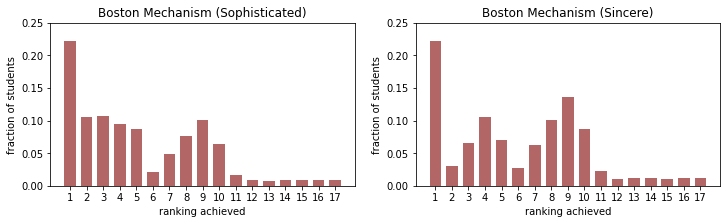
\includegraphics[width=0.99\textwidth]{../figures/BM_frac_choice_p2.png}\\
  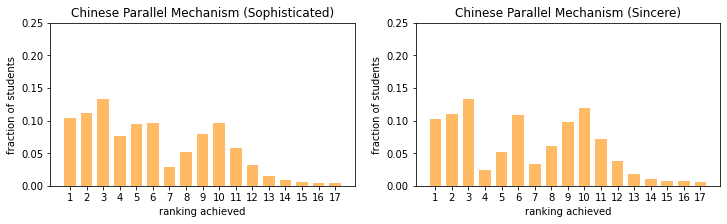
\includegraphics[width=0.99\textwidth]{../figures/CP_frac_choice_p2.png}\\
  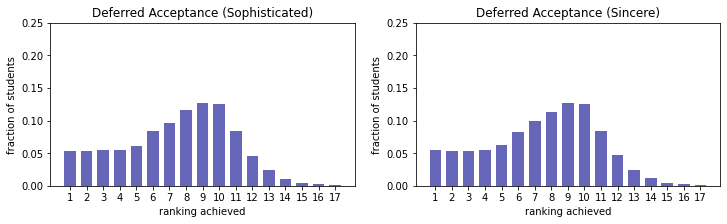
\includegraphics[width=0.99\textwidth]{../figures/DA_frac_choice_p2.png}
  \caption{Fraction of students who get their $k$th favorite school in Deferred Acceptance and Boston Mechanism}
  \label{fig:figure1}
\end{figure}

Figure \ref{fig:figure1} compares the fraction of sincere and sophisticated students who get into their $k$th favorite schools under true preference. 

Unsurprisingly, the distributions for sophisticated and sincere students are almost identical under DA, since both types of students use the same, truthful strategy. 

On the contrary, the distributions differs noticeably under Boston and Chinese Parallel. In the Boston Mechanism, while the fraction is similar with respect to the top choice, sophisticated students are more likely than sincere students to get into their second or third favorite school. Specifically, approximately 11\% of sophisticated students get their second and third choice, but the numbers are 3\% and 6\% for sincere students. These patterns are quite intuitive given the misreports we use in simulation. Both misreports report first choice truthfully if it is safe. Misreport 2 also lists an unsafe favorite as first choice, leaving sophisticated student plenty of opportunities to get their favorite school, on par with the chances for sincere students. Both misreports also aim to secure one of desirable but unpopular schools as a backup, thereby increase the probability for sophisticated students to get their true second and third choices, leading to the high bar for position 2 and 3 in the plot. However, this improvement for sophisticated students are at the expense of sincere students losing priority at their top choices. 

The Chinese Parallel exhibit similar unfairness between sophisticated and sincere student, but to a lesser extent. The fraction of sophisticated and sincere students who receive their top three true preferences are identical, both at 10\%, 11\%, and 13\% respectively. The difference is the most salient at position 4 and 5, which is also a direct consequence of the misreport we adopt. Sophisticated students in our simulation prioritize reporting a safe fourth/fifth favorite school as their third choice to secure a spot in the first round of Chinese Parallel, leading to a systematic higher probability of getting in one of these schools. Again, sincere students are made worse off, and have to resort to a less desirable option. 

Based on Figure \ref{fig:figure1}, DA is unambiguously the best at providing equal education opportunities to sophisticated and sincere students. Chinese Parallel is a distant second---slightly better than Boston for its equal chances for both types of students to get their 3 favorite schools.

In addition, we also compare the average and standard deviation of the ordinal ranks of students' final match under the three mechanisms in Figure \ref{fig:figure2}. In each simulation iteration, we compute the average ordinal rank (standard deviation of ranks) of students' final matches under their true preferences. Then we take an average across all simulation iterations to get the height of each bar. The error bar is $\pm 1.96$ standard deviation of the mean across iterations. 
\begin{figure}[h]
  \centering
  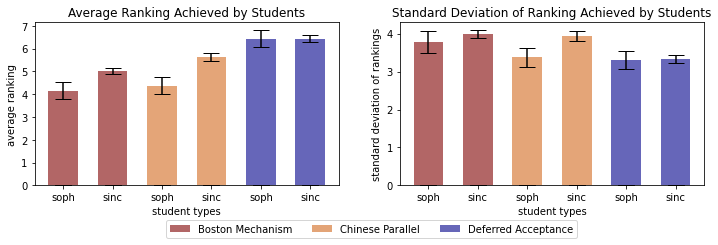
\includegraphics[width=0.99\textwidth]{../figures/DABMCP_rank_ave_std_p2.png}
  \caption{Average and standard deviation of the ordinal ranks of students' final match under true preference}
  \label{fig:figure2}
\end{figure}
The difference in term of ranking received by an average student is statistically significant in both Boston and Chinese Parallel. The magnitude is slightly larger in Chinese Parallel at 1.26, compared with a difference of 0.86 in the Boston Mechanism. The large difference in Chinese Parallel might be due to a large fraction of sincere students losing there fourth or fifth school as shown in Figure \ref{fig:figure1}.

In terms of standard deviation of rankings, Chinese Parallel appears to treat sophisticated and sincere students more unfairly than Boston. Sincere students suffer from a greater variability of final school ranks. Larger standard deviation may be especially undesirable for families from a lower socioeconomic class, since they may not afford a school far from home or their part-time working locations. 

Taken together, the Boston Mechanism and the Chinese Parallel Mechanism appear to be treating sophisticated and sincerely equally unfair in terms of final outcomes. 


% This may appears to contradict the theoretical results that Chinese Parallel is less manipulable than Boston Mechanism. However, we would like to clarify the defenit

However, we would like point out that our simulation does not address the manipulability of Chinese Parallel and Boston. What we have shown only speaks to the welfare difference \textit{conditional} on people strategizing against the system. The result does not touch on how likely it is for individuals in real life to choose to strategize in Chinese Parallel. In fact, \cite{chen2013boston} show in experiments that more people report their top choices truthfully in Chinese Parallel than in Boston. Our simulation keeps the number of sophisticated students constant across mechanisms, ignoring the equilibrium effect altogether. As a result, a real life study may well find that, albeit on a slightly different measure, Chinese Parallel is more fair than Boston. 


\subsection{Pareto Efficiency Comparison}
In this section, we compare the overall welfare achieved under the three mechanisms.

Figures \ref{fig:figure1} and \ref{fig:figure2} already allude to the relatively higher pareto efficiency in Boston and Chinese Parallel. For instance, in Figure \ref{fig:figure1}, we see that the fraction of sophisticated and sincere students who get into their favorite school are both much higher in Boston than in DA; the fraction students who get into their top three favorite schools are also noticeably higher in Chinese Parallel than in DA. Similarly, in Figure \ref{fig:figure2}, both sophisticated and sincere students achieve the least favorable rankings in DA. 

\begin{figure}[h]
  \centering
  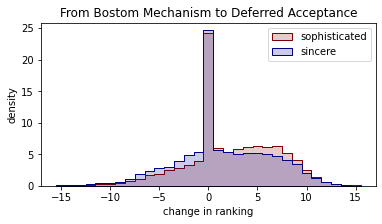
\includegraphics[width=0.49\textwidth]{../figures/BM2DA_rank_change_hist_p2.png}
  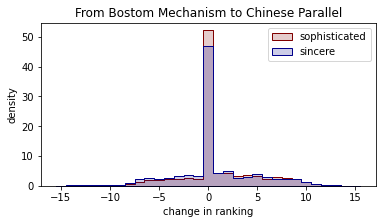
\includegraphics[width=0.49\textwidth]{../figures/BM2CP_rank_change_hist_p2.png}
  \caption{Distribution of change in outcome ranking from the Boston Mechanism to Deferred Acceptance for sophisticated and sincere students}
  \label{fig:figure3}
\end{figure}

Figure \ref{fig:figure3} attempts to compare the welfare comparison more clearly. We take the Boston Mechanism as the baseline, and examine the welfare change switching from Boston to DA (Chinese Parallel).
Use the plot on the left as an sample, we compute the ranking of matched schools under students' true preference in Deferred Acceptance, and minus the ranking achieved in the Boston Mechanism in each iteration. We then pool the difference in ranking across iterations and plot the distribution for sophisticated and sincere students separately. Note that a positive change means that the outcome ranking in Deferred Acceptance is less favorable than that in the Boston Mechanism. 

We make three major observations on the switch from Boston to DA:
First, approximately 25\% of the students have the same matching in Boston and in DA. 
Second, the majority of students achieve a more favorable outcome Boston than in DA. This is evident by the larger area under the curve  when $x > 0$. 
Third, sophisticated students tend to prefer Boston. A larger fraction of sophisticated students suffer a loss switching to Deferred Acceptance. This is as expected since Deferred Acceptance levels the playing field for sincere and sophisticated students. 

The switch from Boston to Chinese Parallel is similar qualitative. However, the fraction of students who get the same outcome in both mechanisms is much larger at approximately 50\%, and sophisticated students do not appear to be systematically more severely harmed by the switch. 

To quantify the change in welfare, we compute the fraction of students who are strictly better off switching from Boston to DA (Chinese Parallel) in each simulation. Averaged over 100 iterations, only 25.4\% of students are better off switching to DA. Specifically, 19.4\% of sophisticated students and 26.9\% of sincere students are happy about the change. The numbers are lower for Chinese Parallel. 21.4\% of students are better off switching to Chinese Parallel; 21.7\% of sophisticated students and 21.4\% of sincere students are happy about the change. To show a more complete view on the welfare comparison, if we include students who are \textit{indifferent} about the switch in this calculation, 50.1\% and 68.0\% of students weakly prefer switching to DA and Chinese Parallel, respectively. 

Finally, we calculate the decrease in ranking for an average student switching from Boston to DA (Chinese Parallel). On average, each student is worse off by approximately 1.60 positions switching to DA; and by approximately 0.53 positions switching to Chinese Parallel.

The loss in welfare switching to DA is surprisingly large in our opinion, \TODO{begs the question why Boston switched to DA}.


\subsection{Stability Comparison}
The overall better outcome in the Boston Mechanism comes at the cost of instability. 

For this analysis, we count the number of blocking pairs in the final matching, where school $j$ and student $i$ is a blocking pair if they prefer each other to their match assigned by the mechanism. See Figure \ref{fig:figure3}.

\begin{figure}[h]
  \centering
  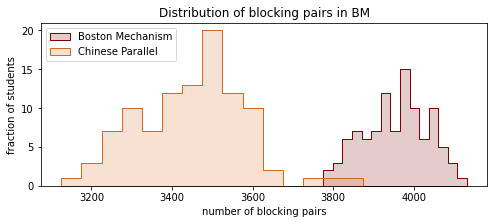
\includegraphics[width=0.99\textwidth]{../figures/blocking_pairs_hist_p2.png}
  \caption{Distribution of the number of blocking pairs in the Boston Mechanism and in Chinese Parallel}
  \label{fig:figure4}
\end{figure}

All matches given by Deferred Acceptance are stable, so there is 0 blocking pairs.\footnote{We did check that there is no block pair in our Deferred Acceptance outcomes just to make sure :D.}

The Boston Mechanism, on the other hand, is quite unstable. Across 100 iterations, there are on average 3955 blocking pairs among a total of $1884\times17=32,028$ school-student pairs. More than $12\%$ of the pairs are blocking pairs. Chinese Parallel is much better with an average of 3448 (also approximately 11\%) blocking pairs. 

\subsection{Effect of Varying the Number of Sophisticated Students}
The final section concerns the scenario in which sincere students become sophisticated as they are informed of the benefit of strategizing. As the result, the number of sophisticated students may increase each year after adoption of Boston or Chinese Parallel. We would like to explore whether having more sophisticated students affect the outcomes in Boston and Chinese Parallel. 

We set the fraction of sophisticated students to be 80\% and rerun all the simulations. In general, the analysis results remain similar to what we show above.\footnote{In the interest of space, we do not present the figures in this paper, since they are mostly similar to previous figures to human eye. Interested readers can refer to our code repository for this cut of figures and statistics at \url{https://github.com/lotusxia/school-choice-136}.} Below, we highlight two worth-noting observations. 

First, a slightly higher fraction (72\% compared with 69\%) of students weakly prefer Chinese Parallel to Boston. Sophisticated students especially favor the change--73\% and 68\% of sophisticated and sincere students weakly prefer the change. The numbers are almost identical for sophisticated and sincere students when the fraction of sophisticated student is small. Without reading too much into the results, we speculate that sophisticated students have a spillover effect in Chinese Parallel, at least under the misreport used in our simulation. 

Second, the final matching becomes noticeably more stable when more people become sophisticated. Figure \ref{fig:figure5} plots the new distributions. \TODO{why...?}

\begin{figure}[h]
  \centering
  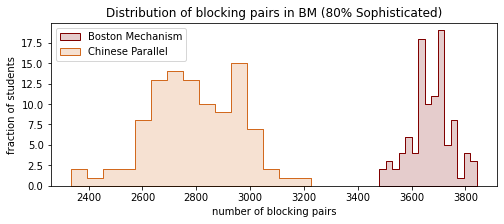
\includegraphics[width=0.99\textwidth]{../figures/blocking_pairs_hist_p8.png}
  \caption{Distribution of the number of blocking pairs in the Boston Mechanism and in Chinese Parallel when the fraction of sophisticated students is 80\%}
  \label{fig:figure5}
\end{figure}


\section{Conclusion}
\TODO{}
Our analysis partly explains why BM is used widely throughout the US. It provides the best welfare to student in general. This is consistent with theory that BM is Pareto optimal for students with respect to the reported preferences. 

A couple other takeaways from these analyses:
\begin{enumerate}
	\item the tradeoff between welfare, fairness, and stability is difficult.
	\item DA may not be as good as advocated by theorist since it comes at a great loss of welfare. 
	\item CP and BM does not seem to differ by that much. They are similar in terms of unfairness. BM is better at welfare whereas CP is better at stability.
	\item Depending on what is most valued by people in different areas, policy maker should plan accordingly. For instance, in places with big difference in socio-economic status, DA may be the best option. If policy maker end up using BM or CP, they should consider make the misreport strategy public and easily accessible so that sincere people can come sophisticated and not be harmed.
\end{enumerate}





\newpage
\bibliographystyle{ecca}
\bibliography{main.bib}

\end{document}
